% !TEX encoding = UTF-8 Unicode

\documentclass[a4paper]{article}

\usepackage{color}
\usepackage{xcolor}
\usepackage{url}
\usepackage[T2A]{fontenc} % enable Cyrillic fonts
\usepackage[utf8]{inputenc} % make weird characters work
\usepackage{graphicx}
\usepackage{amsthm}
\usepackage{amsmath}
\usepackage{booktabs,hhline}
\usepackage{caption}
\usepackage{subcaption}

\usepackage{multirow}       % used for making multirow tables (Nemanja)

%\usepackage[english,serbian]{babel}
\usepackage[english,serbianc]{babel} %ukljuciti babel sa ovim opcijama, umesto gornjim, ukoliko se koristi cirilica

\usepackage[unicode]{hyperref}
\hypersetup{colorlinks,citecolor=green,filecolor=green,linkcolor=blue,urlcolor=blue}

\newtheorem{primer}{Пример}[section] %ćirilični primer
%\newtheorem{primer}{Primer}[section]

\newtheorem{definic}{Дефиниција}
\newcommand{\norm}[1]{\left\lVert#1\right\rVert}

\begin{document}

%TODO smisliti naslov
\title{Решавање неких логичких игара користећи СМТ решаваче\\ \small{Семинарски рад у оквиру курса\\Аутоматско резоновање\\ Математички факултет}}

\author{Немања Мићовић, Лазар Ранковић\\nmicovic@outlook.com, lazar.rankovic@outlook.com}
\date{}
\maketitle

\abstract{
    dodati abstrakt dodati abstrakt dodati abstrakt dodati abstrakt dodati abstrakt
    dodati abstrakt dodati abstrakt dodati abstrakt dodati abstrakt dodati abstrakt
}

\tableofcontents

\newpage

% ---------------------------------------------------------------------------------------------------------------------
\section{Логичке игре}
% ---------------------------------------------------------------------------------------------------------------------
Логичке игре за собом имају дубоку традицију и историју, а упркос страховито брзом развоју технологије у последњих
неколико година, и даље поседују велику популарност. Разлог за њихову популарност јесте често једноставност правила
и неочекивана комплекност која уме да заинтригира људе. У многим часописима се редовно штампају игре као што је судоку
(приказан на слици \ref{fig:sudoku}).

Логичке игре односно загонетке су погодне за математички опис користећи логику и представљају чест пример примене
САТ и СМТ решавача за генерисање инстанци проблема, решавање и валидацију да ли је решење јединствено.

\begin{figure}[h!]
    \begin{center}
        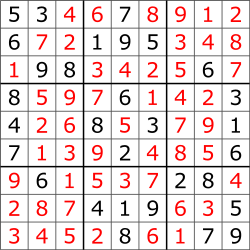
\includegraphics[scale=0.4]{./slike/sudoku.png}
    \end{center}
    \caption{Судоку}
    \label{fig:sudoku}
\end{figure}

% ---------------------------------------------------------------------------------------------------------------------
\section{СМТ решавачи}
% ---------------------------------------------------------------------------------------------------------------------

% ---------------------------------------------------------------------------------------------------------------------
\section{Решавање логичких игара користећи СМТ решаваче}
% ---------------------------------------------------------------------------------------------------------------------

% -------------------------------------------------------------------------------------------------
\subsection{Логичка игра Три суседне}
% -------------------------------------------------------------------------------------------------
Логичка игра \emph{Три судедне} се састоји из матрице поља димензије $n \times n$. На почетку игре,
поља су обојена у плаво, бело и сиво. Поља која су обојена у сиво, играч може да промени у плава или бела,
док оригинална плава и бела поља не може да мења. Ово ћемо звати \emph{почетно стање игре}.

Циљ игре је да играч сва сива поља обоји у плаво или бело при чему морају да важе следећа ограничења:
\begin{itemize}
    \item Не постоје три суседна поља у истој врсти која су обојена истом бојом (услов 1)
    \item Не постоје три суседна поља у истој колони која су обојена истом бојом (услов 2)
    \item У свим врстама мора бити једнак број плавих и белих поља (услов 3)
    \item У свим колонама мора бити једнак број плавих и белих поља (услов 4)
\end{itemize}

Стање у којем се налази табла (матрица) игре када је игра решена назваћемо \emph{задовољено стање игре}. 

На слици \ref{fig:threeway_original} је приказанo почетно стање игре, а на слици \ref{fig:threeway_solved} решена инстанца игре игрe \emph{Три суседне}.

\begin{figure}
\centering
\begin{minipage}{.5\textwidth}
	\centering
	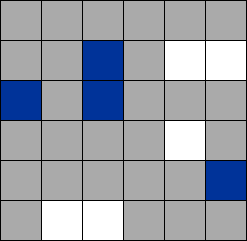
\includegraphics[width=.4\linewidth]{./slike/three_way_original.png}
	\captionof{figure}{Почетно стање игре}
	\label{fig:threeway_original}
\end{minipage}%
\begin{minipage}{.5\textwidth}
  \centering
  
\includegraphics[width=.4\linewidth]{./slike/three_way_solved.png}
  \captionof{figure}{Задовољено стање игре}
  \label{fig:threeway_solved}
\end{minipage}
\end{figure}

\subsubsection{Огранињења}
Како би СМТ решавачем генерисали решења биће нам потребно кодирање претходно наведених услова. Таблу игре
ћемо кодирати користећи $n \times n$ променљивих које ћемо означавати са $x_{i, j}$.


\[
    x_{i, j} = \left\{\begin{array}{lr}
        -1, & \text{за бела поља} \\
        0, & \text{за сива поља } \\
        1, & \text{за плава поља } 
    \end{array}\right\}
\]

При чему важи:
$$ I = \{0, 1, ..., n-1\} $$
$$ J = \{0, 1, ..., n-1\} $$
$$ T = \{-2, -1, 0, 1, 2\} $$
$$ i \in I, j \in J $$

\paragraph{Услов 1}
Кодирање услова 1 изводимо захтевом да збир три суседна поља у врсти мора припадати скупу $T$. Како имамо $n$ врсти,
при чему по свакој врсти имамо $n-2$ ограничења, добијамо $n(n-2)$ ограничења.

$$ x_{i,j} + x_{i, j+1} + x_{i, j+2} \in T $$
$$ i \in \{0, 1, ..., n-1\} $$
$$ j \in \{0, 1, ..., n-3\} $$

\paragraph{Услов 2}
Услов 2 је симетричан услову 1 тако да се добија још $n(n-2)$ додатних ограничења облика:
$$ x_{i, j} + x_{i+1, j} + x_{i+2, j} \in T $$
$$ i \in \{0, 1, ..., n-3\} $$
$$ j \in \{0, 1, ..., n-1\} $$

\paragraph{Услов 3}
Намећемо ограничење да збир у свакој врсти мора бити 0. Како променљиве $x_{i, j}$ имају вредност 1 или -1, ограничење
имплицира једнак број плавих и белих поља у врсти. Ако је број врсти $n$ тиме добијамо још $n$ ограничења облика:
$$ x_{0, 0} + x_{0, 1} + ... + x_{0, n-1} = 0 $$
$$ x_{1, 0} + x_{1, 1} + ... + x_{1, n-1} = 0 $$
$$ ...  $$
$$ x_{n-1, 0} + x_{n-1, 1} + ... + x_{n-1, n-1} = 0 $$

\paragraph{Услов 4}
Услов 4 је симетричан услову 3 те добијамо додатних $n$ ограничења облика:
$$ x_{0, 0} + x_{0, 1} + ... + x_{0, n-1} = 0 $$
$$ x_{0, 1} + x_{1, 1} + ... + x_{n-1, 1} = 0 $$
$$ ...  $$
$$ x_{0, n-1} + x_{1, n-1} + ... + x_{n-1, n-1} = 0 $$

\paragraph{Услови домена}
Решавачу је потребно наметнути дозвољене вредности за сваку од променљивих. Како решавање логичке игре започињемо
од унапред задатог стања (нека поља су већ обојена и не могу се мењати), имамо две врсте ограничења.

Оригинално задата плава и бела поља, решавачу намећемо вредности променљивих 1 или -1. Ако је на пример
поље (0, 3) обојено у плаво, а поље (3, 2) у бело мора важити:
$$ x_{0, 3} = 1 $$
$$ x_{3, 2} = -1 $$

За свако сиво обојено поље $x_{i, j}$, намећемо ограничења да вредности могу бити или -1 или 1.
$$
	x_{i, j} \neq 0 \land -1 \geq x_{i, j} \leq 1	
$$

Како имамо $n \times n$ променљивих, добијамо још $n \times n$ услова.

\subsubsection{Питање јединствености решења}
Како би се показала и доказала јединственост решењa, може се користити решавач да се добију вредности променљивих, а да се након тога
додају ограничења да променљиве не могу узети вредности које представљају решења. Овде треба бити опрезан и приметити да само оригинална сива
поља треба ограничити, а плава и бела (из почетног стања игре) не.

\subsection{Yices program}
Написан је c++ програм који за дато почетно стање игре генерише претходно наведена ограничења у синтакси погодној за
yices смт решавач. Следи генерисани код за једну од инстанци игре.

\begin{verbatim}
(set-logic QF_LIA)
(declare-fun x0_0 () Int)
(declare-fun x0_1 () Int)
(declare-fun x0_2 () Int)
(declare-fun x0_3 () Int)
(declare-fun x0_4 () Int)
(declare-fun x0_5 () Int)
(declare-fun x1_0 () Int)
(declare-fun x1_1 () Int)
(declare-fun x1_2 () Int)
(declare-fun x1_3 () Int)
(declare-fun x1_4 () Int)
(declare-fun x1_5 () Int)
(declare-fun x2_0 () Int)
(declare-fun x2_1 () Int)
(declare-fun x2_2 () Int)
(declare-fun x2_3 () Int)
(declare-fun x2_4 () Int)
(declare-fun x2_5 () Int)
(declare-fun x3_0 () Int)
(declare-fun x3_1 () Int)
(declare-fun x3_2 () Int)
(declare-fun x3_3 () Int)
(declare-fun x3_4 () Int)
(declare-fun x3_5 () Int)
(declare-fun x4_0 () Int)
(declare-fun x4_1 () Int)
(declare-fun x4_2 () Int)
(declare-fun x4_3 () Int)
(declare-fun x4_4 () Int)
(declare-fun x4_5 () Int)
(declare-fun x5_0 () Int)
(declare-fun x5_1 () Int)
(declare-fun x5_2 () Int)
(declare-fun x5_3 () Int)
(declare-fun x5_4 () Int)
(declare-fun x5_5 () Int)
(assert
    (and 
        ;; Ограничења домена
        (and (<= (- 1) x0_0)(>= 1 x0_0)(distinct 0 x0_0))
        (and (<= (- 1) x0_1)(>= 1 x0_1)(distinct 0 x0_1))
        (= x0_2 1)
        (and (<= (- 1) x0_3)(>= 1 x0_3)(distinct 0 x0_3))
        (and (<= (- 1) x0_4)(>= 1 x0_4)(distinct 0 x0_4))
        (and (<= (- 1) x0_5)(>= 1 x0_5)(distinct 0 x0_5))
        (and (<= (- 1) x1_0)(>= 1 x1_0)(distinct 0 x1_0))
        (= x1_1 1)
        (and (<= (- 1) x1_2)(>= 1 x1_2)(distinct 0 x1_2))
        (and (<= (- 1) x1_3)(>= 1 x1_3)(distinct 0 x1_3))
        (= x1_4 (- 1))
        (and (<= (- 1) x1_5)(>= 1 x1_5)(distinct 0 x1_5))
        (and (<= (- 1) x2_0)(>= 1 x2_0)(distinct 0 x2_0))
        (= x2_1 (- 1))
        (and (<= (- 1) x2_2)(>= 1 x2_2)(distinct 0 x2_2))
        (and (<= (- 1) x2_3)(>= 1 x2_3)(distinct 0 x2_3))
        (and (<= (- 1) x2_4)(>= 1 x2_4)(distinct 0 x2_4))
        (and (<= (- 1) x2_5)(>= 1 x2_5)(distinct 0 x2_5))
        (= x3_0 (- 1))
        (and (<= (- 1) x3_1)(>= 1 x3_1)(distinct 0 x3_1))
        (= x3_2 1)
        (and (<= (- 1) x3_3)(>= 1 x3_3)(distinct 0 x3_3))
        (= x3_4 (- 1))
        (and (<= (- 1) x3_5)(>= 1 x3_5)(distinct 0 x3_5))
        (and (<= (- 1) x4_0)(>= 1 x4_0)(distinct 0 x4_0))
        (and (<= (- 1) x4_1)(>= 1 x4_1)(distinct 0 x4_1))
        (and (<= (- 1) x4_2)(>= 1 x4_2)(distinct 0 x4_2))
        (and (<= (- 1) x4_3)(>= 1 x4_3)(distinct 0 x4_3))
        (and (<= (- 1) x4_4)(>= 1 x4_4)(distinct 0 x4_4))
        (= x4_5 (- 1))
        (and (<= (- 1) x5_0)(>= 1 x5_0)(distinct 0 x5_0))
        (= x5_1 1)
        (= x5_2 1)
        (and (<= (- 1) x5_3)(>= 1 x5_3)(distinct 0 x5_3))
        (= x5_4 1)
        (and (<= (- 1) x5_5)(>= 1 x5_5)(distinct 0 x5_5))

        ;; У истој врсти три суседна поља не смеју бити сте боје
        (and (> (+ x0_0 x0_1 x0_2) (- 3))(< (+ x0_0 x0_1 x0_2) 3))
        (and (> (+ x0_0 x0_1 x0_2) (- 3))(< (+ x0_0 x0_1 x0_2) 3))
        (and (> (+ x0_1 x0_2 x0_3) (- 3))(< (+ x0_1 x0_2 x0_3) 3))
        (and (> (+ x0_1 x0_2 x0_3) (- 3))(< (+ x0_1 x0_2 x0_3) 3))
        (and (> (+ x0_2 x0_3 x0_4) (- 3))(< (+ x0_2 x0_3 x0_4) 3))
        (and (> (+ x0_2 x0_3 x0_4) (- 3))(< (+ x0_2 x0_3 x0_4) 3))
        (and (> (+ x0_3 x0_4 x0_5) (- 3))(< (+ x0_3 x0_4 x0_5) 3))
        (and (> (+ x0_3 x0_4 x0_5) (- 3))(< (+ x0_3 x0_4 x0_5) 3))
        (and (> (+ x1_0 x1_1 x1_2) (- 3))(< (+ x1_0 x1_1 x1_2) 3))
        (and (> (+ x1_0 x1_1 x1_2) (- 3))(< (+ x1_0 x1_1 x1_2) 3))
        (and (> (+ x1_1 x1_2 x1_3) (- 3))(< (+ x1_1 x1_2 x1_3) 3))
        (and (> (+ x1_1 x1_2 x1_3) (- 3))(< (+ x1_1 x1_2 x1_3) 3))
        (and (> (+ x1_2 x1_3 x1_4) (- 3))(< (+ x1_2 x1_3 x1_4) 3))
        (and (> (+ x1_2 x1_3 x1_4) (- 3))(< (+ x1_2 x1_3 x1_4) 3))
        (and (> (+ x1_3 x1_4 x1_5) (- 3))(< (+ x1_3 x1_4 x1_5) 3))
        (and (> (+ x1_3 x1_4 x1_5) (- 3))(< (+ x1_3 x1_4 x1_5) 3))
        (and (> (+ x2_0 x2_1 x2_2) (- 3))(< (+ x2_0 x2_1 x2_2) 3))
        (and (> (+ x2_0 x2_1 x2_2) (- 3))(< (+ x2_0 x2_1 x2_2) 3))
        (and (> (+ x2_1 x2_2 x2_3) (- 3))(< (+ x2_1 x2_2 x2_3) 3))
        (and (> (+ x2_1 x2_2 x2_3) (- 3))(< (+ x2_1 x2_2 x2_3) 3))
        (and (> (+ x2_2 x2_3 x2_4) (- 3))(< (+ x2_2 x2_3 x2_4) 3))
        (and (> (+ x2_2 x2_3 x2_4) (- 3))(< (+ x2_2 x2_3 x2_4) 3))
        (and (> (+ x2_3 x2_4 x2_5) (- 3))(< (+ x2_3 x2_4 x2_5) 3))
        (and (> (+ x2_3 x2_4 x2_5) (- 3))(< (+ x2_3 x2_4 x2_5) 3))
        (and (> (+ x3_0 x3_1 x3_2) (- 3))(< (+ x3_0 x3_1 x3_2) 3))
        (and (> (+ x3_0 x3_1 x3_2) (- 3))(< (+ x3_0 x3_1 x3_2) 3))
        (and (> (+ x3_1 x3_2 x3_3) (- 3))(< (+ x3_1 x3_2 x3_3) 3))
        (and (> (+ x3_1 x3_2 x3_3) (- 3))(< (+ x3_1 x3_2 x3_3) 3))
        (and (> (+ x3_2 x3_3 x3_4) (- 3))(< (+ x3_2 x3_3 x3_4) 3))
        (and (> (+ x3_2 x3_3 x3_4) (- 3))(< (+ x3_2 x3_3 x3_4) 3))
        (and (> (+ x3_3 x3_4 x3_5) (- 3))(< (+ x3_3 x3_4 x3_5) 3))
        (and (> (+ x3_3 x3_4 x3_5) (- 3))(< (+ x3_3 x3_4 x3_5) 3))
        (and (> (+ x4_0 x4_1 x4_2) (- 3))(< (+ x4_0 x4_1 x4_2) 3))
        (and (> (+ x4_0 x4_1 x4_2) (- 3))(< (+ x4_0 x4_1 x4_2) 3))
        (and (> (+ x4_1 x4_2 x4_3) (- 3))(< (+ x4_1 x4_2 x4_3) 3))
        (and (> (+ x4_1 x4_2 x4_3) (- 3))(< (+ x4_1 x4_2 x4_3) 3))
        (and (> (+ x4_2 x4_3 x4_4) (- 3))(< (+ x4_2 x4_3 x4_4) 3))
        (and (> (+ x4_2 x4_3 x4_4) (- 3))(< (+ x4_2 x4_3 x4_4) 3))
        (and (> (+ x4_3 x4_4 x4_5) (- 3))(< (+ x4_3 x4_4 x4_5) 3))
        (and (> (+ x4_3 x4_4 x4_5) (- 3))(< (+ x4_3 x4_4 x4_5) 3))
        (and (> (+ x5_0 x5_1 x5_2) (- 3))(< (+ x5_0 x5_1 x5_2) 3))
        (and (> (+ x5_0 x5_1 x5_2) (- 3))(< (+ x5_0 x5_1 x5_2) 3))
        (and (> (+ x5_1 x5_2 x5_3) (- 3))(< (+ x5_1 x5_2 x5_3) 3))
        (and (> (+ x5_1 x5_2 x5_3) (- 3))(< (+ x5_1 x5_2 x5_3) 3))
        (and (> (+ x5_2 x5_3 x5_4) (- 3))(< (+ x5_2 x5_3 x5_4) 3))
        (and (> (+ x5_2 x5_3 x5_4) (- 3))(< (+ x5_2 x5_3 x5_4) 3))
        (and (> (+ x5_3 x5_4 x5_5) (- 3))(< (+ x5_3 x5_4 x5_5) 3))
        (and (> (+ x5_3 x5_4 x5_5) (- 3))(< (+ x5_3 x5_4 x5_5) 3))

        ;; У истој колони три суседна поља не смеју бити сте боје
        (and (> (+ x0_0 x1_0 x2_0) (- 3))(< (+ x0_0 x1_0 x2_0) 3))
        (and (> (+ x1_0 x2_0 x3_0) (- 3))(< (+ x1_0 x2_0 x3_0) 3))
        (and (> (+ x2_0 x3_0 x4_0) (- 3))(< (+ x2_0 x3_0 x4_0) 3))
        (and (> (+ x3_0 x4_0 x5_0) (- 3))(< (+ x3_0 x4_0 x5_0) 3))
        (and (> (+ x0_1 x1_1 x2_1) (- 3))(< (+ x0_1 x1_1 x2_1) 3))
        (and (> (+ x1_1 x2_1 x3_1) (- 3))(< (+ x1_1 x2_1 x3_1) 3))
        (and (> (+ x2_1 x3_1 x4_1) (- 3))(< (+ x2_1 x3_1 x4_1) 3))
        (and (> (+ x3_1 x4_1 x5_1) (- 3))(< (+ x3_1 x4_1 x5_1) 3))
        (and (> (+ x0_2 x1_2 x2_2) (- 3))(< (+ x0_2 x1_2 x2_2) 3))
        (and (> (+ x1_2 x2_2 x3_2) (- 3))(< (+ x1_2 x2_2 x3_2) 3))
        (and (> (+ x2_2 x3_2 x4_2) (- 3))(< (+ x2_2 x3_2 x4_2) 3))
        (and (> (+ x3_2 x4_2 x5_2) (- 3))(< (+ x3_2 x4_2 x5_2) 3))
        (and (> (+ x0_3 x1_3 x2_3) (- 3))(< (+ x0_3 x1_3 x2_3) 3))
        (and (> (+ x1_3 x2_3 x3_3) (- 3))(< (+ x1_3 x2_3 x3_3) 3))
        (and (> (+ x2_3 x3_3 x4_3) (- 3))(< (+ x2_3 x3_3 x4_3) 3))
        (and (> (+ x3_3 x4_3 x5_3) (- 3))(< (+ x3_3 x4_3 x5_3) 3))
        (and (> (+ x0_4 x1_4 x2_4) (- 3))(< (+ x0_4 x1_4 x2_4) 3))
        (and (> (+ x1_4 x2_4 x3_4) (- 3))(< (+ x1_4 x2_4 x3_4) 3))
        (and (> (+ x2_4 x3_4 x4_4) (- 3))(< (+ x2_4 x3_4 x4_4) 3))
        (and (> (+ x3_4 x4_4 x5_4) (- 3))(< (+ x3_4 x4_4 x5_4) 3))
        (and (> (+ x0_5 x1_5 x2_5) (- 3))(< (+ x0_5 x1_5 x2_5) 3))
        (and (> (+ x1_5 x2_5 x3_5) (- 3))(< (+ x1_5 x2_5 x3_5) 3))
        (and (> (+ x2_5 x3_5 x4_5) (- 3))(< (+ x2_5 x3_5 x4_5) 3))
        (and (> (+ x3_5 x4_5 x5_5) (- 3))(< (+ x3_5 x4_5 x5_5) 3))

        ;; За сваку врсту мора постојати једнак број плавих и белих поља.
        (= 0 (+ x0_0 x0_1 x0_2 x0_3 x0_4 x0_5))
        (= 0 (+ x1_0 x1_1 x1_2 x1_3 x1_4 x1_5))
        (= 0 (+ x2_0 x2_1 x2_2 x2_3 x2_4 x2_5))
        (= 0 (+ x3_0 x3_1 x3_2 x3_3 x3_4 x3_5))
        (= 0 (+ x4_0 x4_1 x4_2 x4_3 x4_4 x4_5))
        (= 0 (+ x5_0 x5_1 x5_2 x5_3 x5_4 x5_5))

        ;; За сваку колону мора постојати једнак број плавих и белих поља.
        (= 0 (+ x0_0 x1_0 x2_0 x3_0 x4_0 x5_0))
        (= 0 (+ x0_1 x1_1 x2_1 x3_1 x4_1 x5_1))
        (= 0 (+ x0_2 x1_2 x2_2 x3_2 x4_2 x5_2))
        (= 0 (+ x0_3 x1_3 x2_3 x3_3 x4_3 x5_3))
        (= 0 (+ x0_4 x1_4 x2_4 x3_4 x4_4 x5_4))
        (= 0 (+ x0_5 x1_5 x2_5 x3_5 x4_5 x5_5))
))
(check-sat)
(get-value (
        x0_0 x0_1 x0_2 x0_3 x0_4 x0_5
        x1_0 x1_1 x1_2 x1_3 x1_4 x1_5
        x2_0 x2_1 x2_2 x2_3 x2_4 x2_5
        x3_0 x3_1 x3_2 x3_3 x3_4 x3_5
        x4_0 x4_1 x4_2 x4_3 x4_4 x4_5
        x5_0 x5_1 x5_2 x5_3 x5_4 x5_5
    )
)
(exit)
\end{verbatim}

Покретање речавање даје да је проблем задовољив и даје нам вредности променљивих $x_{i, j}$ које представљају
распоред поља.

\begin{verbatim}
sat
((x0_0 1)
 (x0_1 (- 1))
 (x0_2 1)
 (x0_3 (- 1))
 (x0_4 (- 1))
 (x0_5 1)
 (x1_0 (- 1))
 (x1_1 1)
 (x1_2 (- 1))
 (x1_3 1)
 (x1_4 (- 1))
 (x1_5 1)
 (x2_0 1)
 (x2_1 (- 1))
 (x2_2 (- 1))
 (x2_3 1)
 (x2_4 1)
 (x2_5 (- 1))
 (x3_0 (- 1))
 (x3_1 1)
 (x3_2 1)
 (x3_3 (- 1))
 (x3_4 (- 1))
 (x3_5 1)
 (x4_0 1)
 (x4_1 (- 1))
 (x4_2 (- 1))
 (x4_3 1)
 (x4_4 1)
 (x4_5 (- 1))
 (x5_0 (- 1))
 (x5_1 1)
 (x5_2 1)
 (x5_3 (- 1))
 (x5_4 1)
 (x5_5 (- 1)))
\end{verbatim}


% ---------------------------------------------------------------------------------------------------------------------
\section{Закључак}
% ---------------------------------------------------------------------------------------------------------------------
Радови приказани у делу \ref{sec:primene} показали су да област машинског учења може пронаћи примену у области статичке
верификације софтвера. Добијени резултати су били барем упоредиви са другим приступима, а у неким случајевима и доста
бољи. Неки од проблема који се јављају при употреби алгоритама машинског учења јесу неинтерпретабилност добијеног модела и
неегзактна предвиђања које модел врши. Проблем интерпретабилности је превазиђен стаблима одлучивања \cite{KrishnaPW15, Sharma_interpolantsas}
која су позната да дају интерпретабилне моделе, док је проблем неегзактног предвиђања ублажен у раду \cite{Brun04findinglatent}
где се као резултат даје листа програмских својстава које човек анализира. Уколико је неко својство погрешно класификовано,
неће проузроковати велику грешку.

\addcontentsline{toc}{section}{Literatura}
\appendix
\bibliography{seminarski}
\bibliographystyle{plain}


\end{document}
